\chapter{Dr. Kellogg i doktrina o Trojstvu}

Ključni problem Kelloggove kontroverze bili su sentimenti o \emcap{ličnosti Boga}, koji su odstupali od temelja naše vjere, koje je Bog uspostavio na početku našeg rada. Rečeno nam je da \egwinline{Mnoge stvari sličnog karaktera pojaviti će se u budućnosti}[Ms137-1903.10; 1903][https://egwwritings.org/read?panels=p9939.17]. U knjizi, Živi Hram, vidimo sentimente o \emcap{ličnosti Boga} i Njegovoj prisutnosti, koji su odstupali od \emcap{Fundamentalnih Principa}. Ovaj korak nikada nije trebao biti napravljen! Ali postavljamo pitanje, kamo je ovaj korak vodio? Vidjet ćemo pokazatelje da je ovaj korak vodio prema doktrini o Trojstvu. Sestra White je prorekla da će Kelloggov korak voditi prema Omega otpadu. Možemo li vidjeti vezu između Kelloggove kontroverze i doktrine o Trojstvu?

U sljedećem poglavlju želimo vam predstaviti vezu između Kelloggove kontroverze i doktrine o Trojstvu. Važno je naglasiti da Živi Hram ne sadrži ovu doktrinu kako se ona danas vjeruje. Glavni problem s Kelloggovim učenjem bio je \textit{odstupanje} od \emcap{Fundamentalnih Principa}, koji su bili temelj naše vjere. Informacije koje ćemo vam predstaviti otkrivaju da je dr. Kellogg opravdao svoje postupke odstupanjem od temelja kroz svoje vjerovanje u doktrinu o Trojstvu. Ovo nije teško vidjeti kada prepoznamo da su \emcap{Fundamentalni Principi} bili ne-trinitarijanski. Stoga, naš glavni fokus ne bi trebao biti prepoznavanje Trojstva u Kelloggovim argumentima, već u razumijevanju razlika između Kelloggovih učenja i učenja \emcap{Fundamentalnih Principa} u vezi s \egwinline{ličnosti Boga i gdje je Njegova prisutnost}[SpTB02 51.3; 1903][https://egwwritings.org/read?panels=p417.262]. Drugim riječima, koji su to koraci koje je Kellogg napravio odstupajući od temelja naše vjere? Ovaj pristup zagovara Duh Proroštva i pomoći će nam da izbjegnemo spekulacije u vezi s Kelloggovim motivima—pomoći će nam da se usredotočimo na istinu. Ellen White nam govori da u Živom Hramu postoje mnoge dobre stvari, ali su pomiješane s lažnim, obmanjujućim teorijama o \emcap{ličnosti Boga} i \emcap{Krista}.

\begin{figure}[hp]
    \centering
    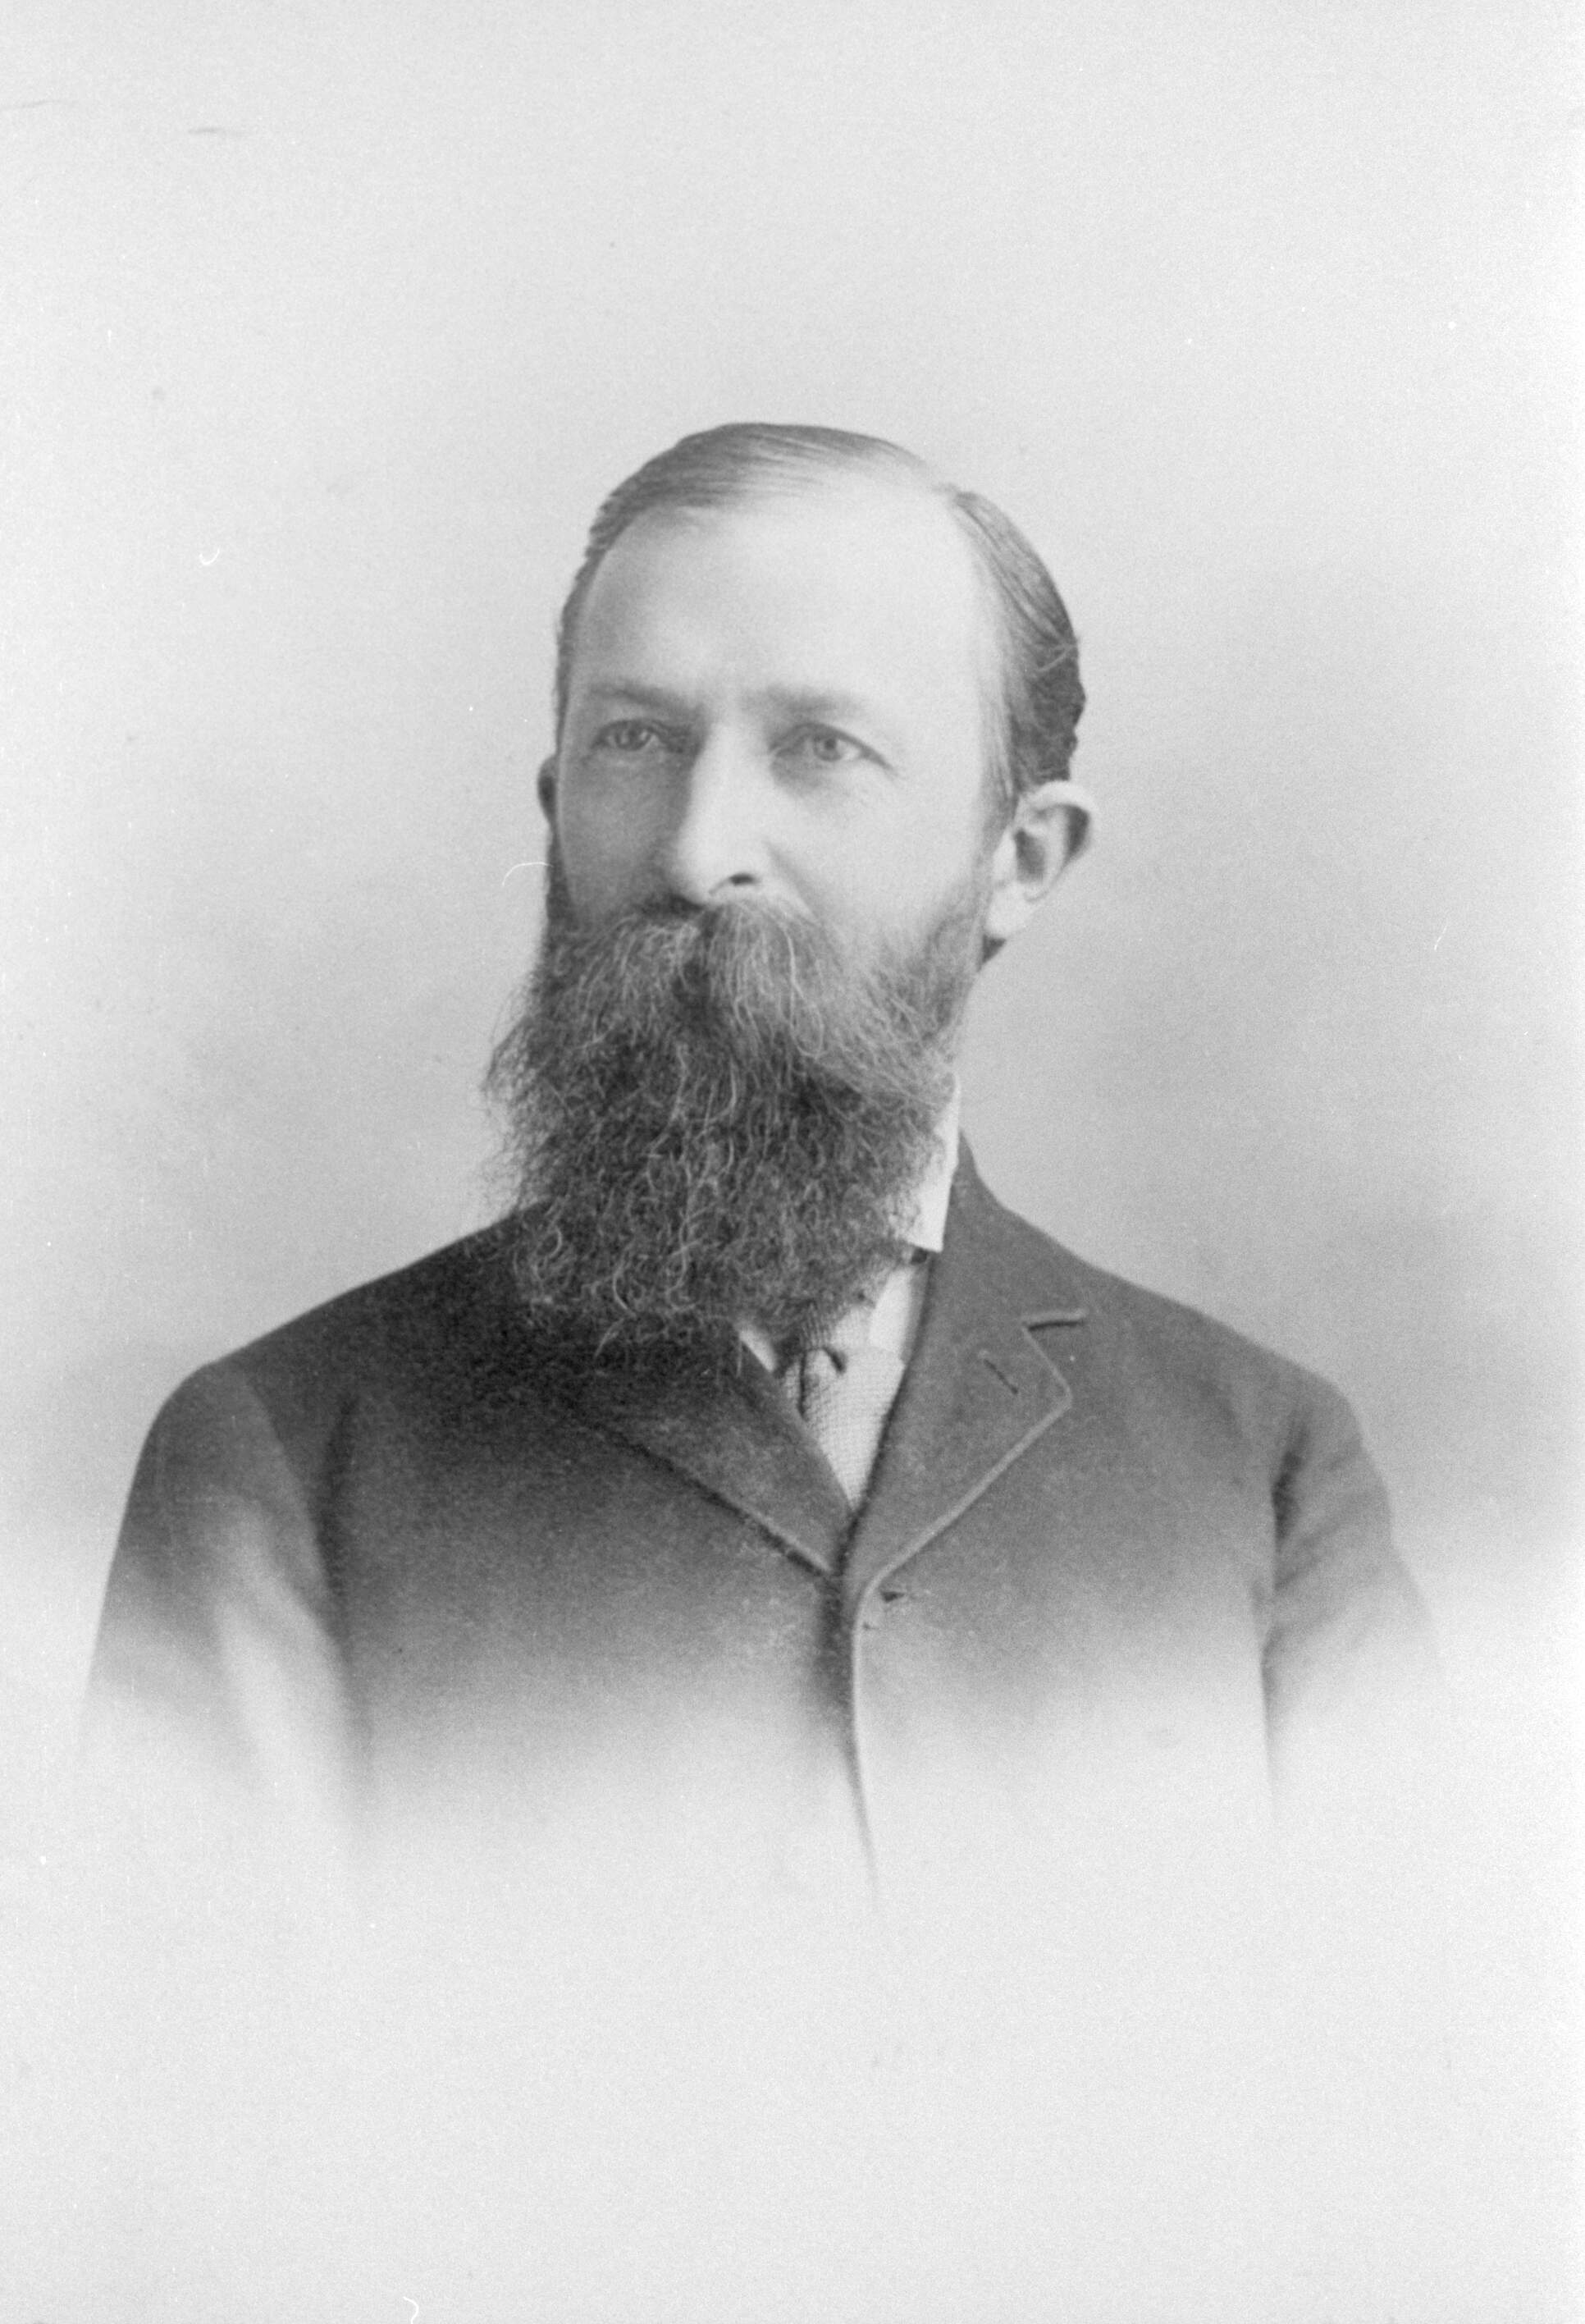
\includegraphics[width=1\linewidth]{images/john-h-kellogg.jpg}
    \caption*{John Harvey Kellogg (1852-1943)}
    \label{fig:john-h-kellogg}
\end{figure}

\egw{\textbf{Knjiga Živi hram sadrži lažne, \underline{obmanjujuće sentimente o ličnosti Boga i Krista}}. Gospodin mi je otvorio pravo značenje tih sentimenta, pokazujući mi da, ako se čvrsto ne odbace, mogu prevariti čak i odabrane. \textbf{Dragocjena istina i lijepe misli isprepletene su s lažnim, obmanjujućim teorijama. Tako je istina korištena za potkrepljivanje \underline{najopasnijih zabluda}. Dragocjene predodžbe o Bogu su tako pogrešno prikazane da izgleda kao da podržavaju laži \underline{koje  je smislio veliki otpadnik}. Sentimenti koji pripadaju Božjim otkrivenjima pomiješani su s zabludama, obmanjujućim teorijama sotonskih djelatnika}.}[Lt146-1905.2; 1905][https://egwwritings.org/read?panels=p9430.8]

\egwnogap{U kontroverzi oko ovih teorija \textbf{tvrdilo se da sam vjerovala i učila iste stvari} koje sam, prema Božjoj upiti, trebala osuditi u knjizi Živi Hram. \textbf{To poričem}. U ime Isusa Krista iz Nazareta, \textbf{kažem da to nije istina}.}[Lt146-1905.3; 1905][https://egwwritings.org/read?panels=p9430.9]

Ova mješavina istine i zablude čini stvar teškom. U očima pristaša doktrine o Trojstvu, problem je isključivo pripisan panteizmu, a dokazi Kelloggovog vjerovanja u doktrinu Trojstva tumače se kao vjerovanje u lažno Trojstvo\footnote{Whidden, Woodrow W. et al. Trojstvo: Razumijevanje Božje ljubavi, Njegova plana spasenja i kršćanskih odnosa. Hagerstown, MD, Review and Herald Pub. Association, 2002., str. 217 orig.}. Ukor sestre White pripisuje se obrani “ispravnog” Trojstva, za koje se pretpostavlja da je vjerovala. Nažalost, takva interpretacija ne priznaje privrženost sestre White \emcap{Fundamentalnih Principa} u vezi \emcap{ličnosti Boga} i Krista, stoga je to pogrešno tumačenje njezinog rada. U nastavku pogledat ćemo povijesne podatke o povezanosti dr. Kellogga s doktrinom o Trojstvu iz perspektive adventističke istine o \emcap{ličnosti Boga}, koja je činila temelj naše vjere. S ovom perspektivom, vjerujemo da će povijesni podaci zasjati u novom svjetlu i potaknuti iskren i konstruktivan dijalog u našoj crkvi.

\section*{Prepiska Dr. Kellogga i brata Butlera}

U nastavku vam ukratko predstavljamo poznatu prepisku između dr. Kellogga i G. I. Butlera o knjizi, Živi Hram. Ovdje vidimo dr. Kelloggove prigovore vezane za kontroverzu. Pisao je bratu Butleru:

\others{Koliko ja mogu razumjeti, \textbf{teškoća} koja se pronalazi \textbf{u ‘Živom Hramu’,} \textbf{sve se može sumirati u sljedećem pitanju}: \textbf{\underline{Je li Sveti Duh osoba}?} Ti kažeš ne. Ja sam pretpostavljao da to proizlazi iz Svetog Pisma iz razloga što se osobna zamjenica ‘on’ koristi onda kada se govori o Svetom Duhu. \textbf{Sestra White koristi zamjenicu ‘on’ i rekla je više puta da je Sveti Duh \underline{treća osoba Božanstva}}. \textbf{Kako Sveti Duh može biti treća osoba, a da uopće ne bude osoba, teško mi je uvidjeti}.}[Letter: J. H. Kellogg to G. I. Butler. Oct 28. 1903][https://static1.squarespace.com/static/554c4998e4b04e89ea0c4073/t/5db9fbc96defed1e45b497a4/1572469707862/1903-10-28-Kellog-to-Butler.pdf]

\begin{figure}[hp]
    \centering
    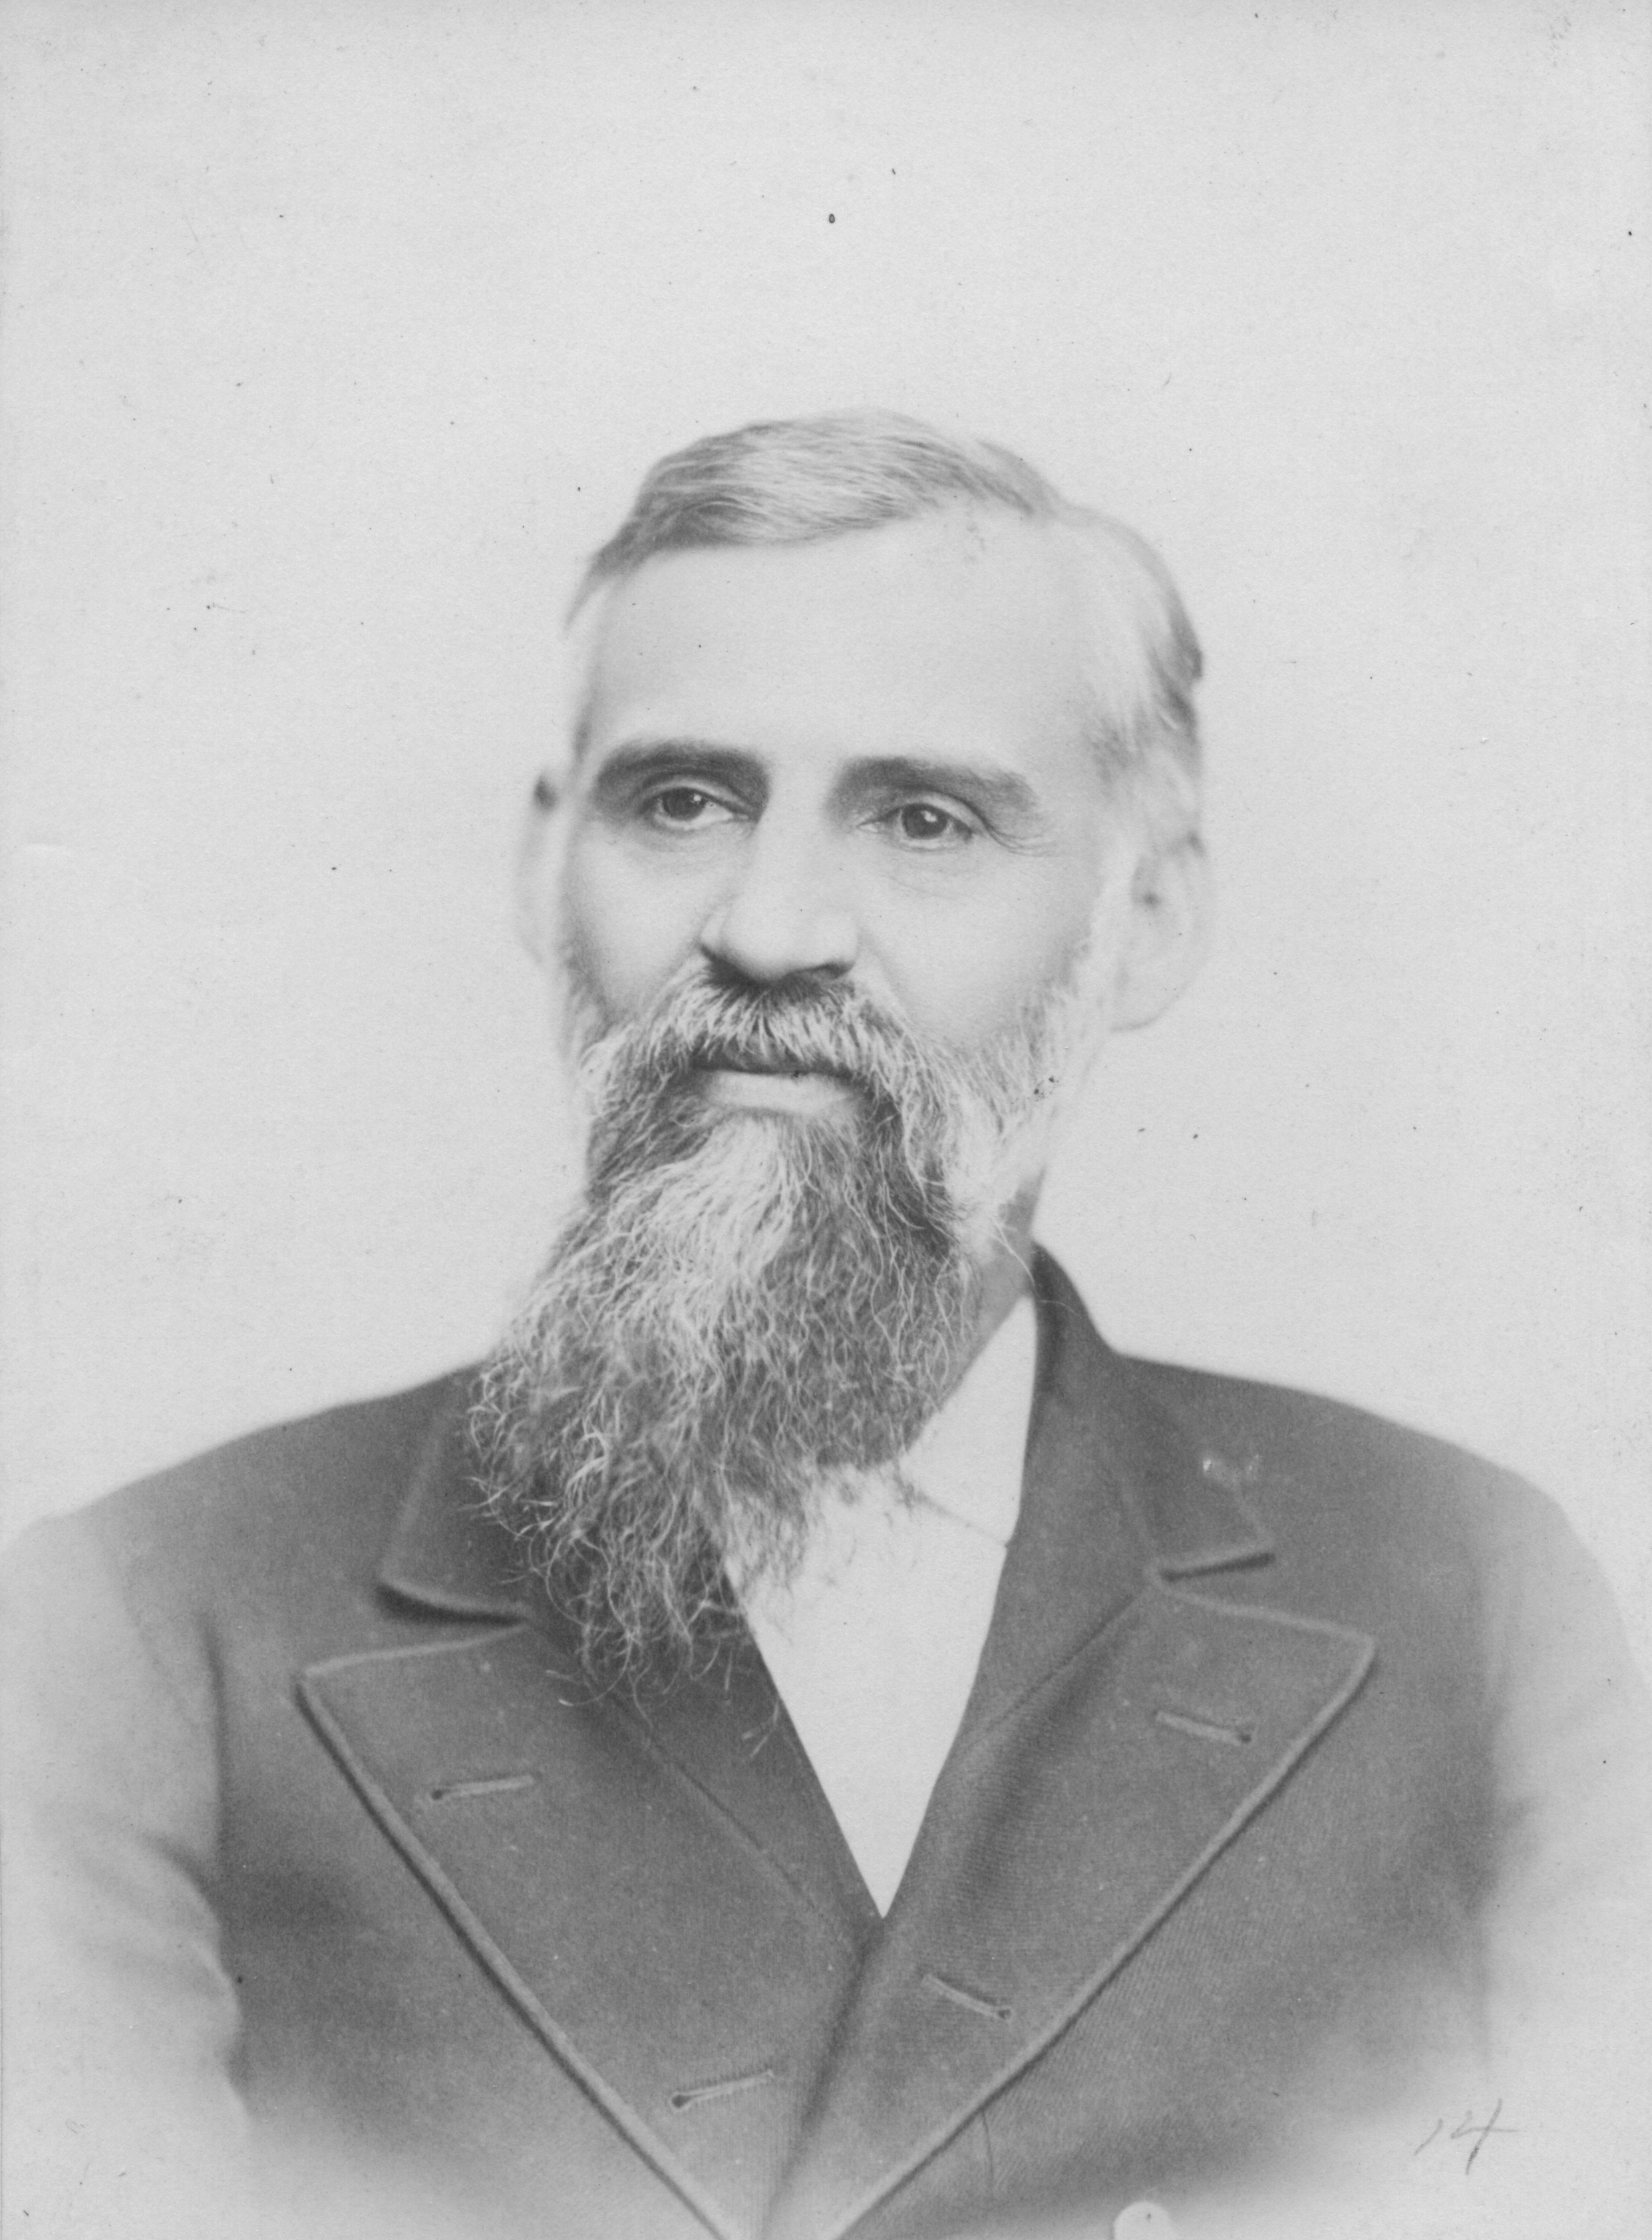
\includegraphics[width=1\linewidth]{images/george-ide-butler.jpg}
    \caption*{George Ide Butler (1834-1918)}
    \label{fig:g-i-butler}
\end{figure}

Prema perspektivi dr. Kellogga, cijeli problem s knjigom ‘Živi Hram’ svodi se na pitanje “\textit{Je li Sveti Duh osoba?}”. Očito je da on ne zagovara neosobnog Boga, kako ga se često optužuje\footnote{Whidden, Woodrow W, et al. \textit{The Trinity : Understanding God's Love, His Plan of Salvation, and Christian Relationships}. Hagerstown, Md, Review And Herald Pub. Association, 2002., p. 217}. Štoviše, čak vjeruje da je Sveti Duh \textit{treća osoba Božanstva}. Također tvrdi da brat Butler ne vjeruje da je Sveti Duh osoba. Problem očito leži u definiciji riječi \textit{‘osoba’}. Po tom pitanju, Kellogg nastavlja:

\others{Ja vjerujem da je Duh Božji ličnost, u što ti ne vjeruješ. Ali ovo je čisto pitanje definicije. \textbf{Ja vjerujem da je Duh Božji ličnost}; ti kažeš: Ne, nije ličnost. Sada je jedini razlog zbog kojeg se mimoilazimo u našim pojmovima o tome \textbf{što je to \underline{ličnost}}. \textbf{Tvoja ideja ličnosti je možda \underline{izvanjska sličnost s osobom} ili ljudskim bićem}.}[Pismo: J. H. Kellogg G. I. Butleru, 28. listopada 1903.][https://static1.squarespace.com/static/554c4998e4b04e89ea0c4073/t/5db9fbc96defed1e45b497a4/1572469707862/1903-10-28-Kellog-to-Butler.pdf]

Brat Butler odgovara:

\others{\textbf{S obzirom na to da ste do sada ti i sestra White bili u potpunom skladu, morat ću u potpunosti napustiti cijelu stvar i ostaviti je tebi i sestri White. \underline{Sestra White kaže da ne postoji potpuni sklad, a ti kažeš da postoji}. \underline{Znam da neke od njenih izjava izgledaju kao da ti daju snažno uporište da tvrdiš da te ona podržava}. Dovoljno sam otvoren da to kažem, ali moram joj dati naklonost sve dok se ona ne odrekne stava da postoji različitost, i ne vjerujem da si u stanju kazati što ona točno misli. \underline{Bog prebiva u nama Svojim Svetim Duhom}, kao Utješitelj, kao Ukoravatelj, ali posebice ovo drugo. Kada dođemo Njemu, mi imamo udjela u Njemu u tom smislu jer Duh proizlazi od Njega; \underline{On proizlazi od Oca i Sina}. To nije neka osoba koja se šeta naokolo ili leti \underline{kao neko doslovno biće}, \underline{u bilo kojem takvom smislu kao što su to Krist i Otac} - ukoliko je to tako onda je to apsolutno izvan mog razumijevanja značenja jezika ili riječi}.}[Pismo: G. I. Butler J. H. Kelloggu, 5. travnja 1904.]

Dana korespondencija je ključna za razumijevanje Kellogove kontroverze. Kellogg je sâm izjavio, \others{sve teškoće mogu se sumirati u sljedećem pitanju: \textbf{Je li Sveti Duh osoba?}} Slično tome, dr. Kellogg je pisao Williamu Whiteu: \others{Vrlo pažljivo sam proučavao da vidim što je \textbf{pravi korijen problema s ‘Živim Hramom’}, i koliko mogu vidjeti \textbf{\underline{cijelo pitanje} se svodi na ovo: \underline{Je li Sveti Duh, osoba}?}}[Pismo: J. H. Kellogg Williamu Whiteu, 28. listopada 1903.][https://drive.google.com/file/d/1\_S4S-Hc0K7Ka8gda9oRhPuAb9XzBTwmb/view] Kako se Kelloggov zaključak može usporediti s uputom nebeskog podrijetla, koje nam jasno kaže da su rasuđivanja u Živom Hramu \egwinline{obična nagađanja vezano za \textbf{ličnost Boga i gdje je Njegova prisutnost}}[SpTB02 51.3; 1904][https://egwwritings.org/read?panels=p417.262]? U spisima Ellen White i pionira, izraz ‘\textit{ličnost Boga}’ odnosi se specifično na ličnost Oca. Dakle, zašto Kellogg tvrdi da je pravi korijen problema ličnost Duha Svetoga, kada je Bog naznačio da je korijen problema ličnost Oca?

Mnogi pretpostavljaju da je dr. Kellogg manipulativan, te izbjegava glavno pitanje. Međutim, pod određenom pretpostavkom, njegovi argumenti o ličnosti Duha Svetoga logički podržavaju njegove kontroverzne poglede na \emcap{ličnost Boga}. Ta pretpostavka postaje očita unutar samih podataka kada pažljivo pratimo njegovo rasuđivanje.

Kao što smo ranije vidjeli, doktrina o \emcap{ličnosti Boga} uči da Bog, Otac, posjeduje oblik—opipljivo, materijalno tijelo. Dr. Kellogg se složio da je ta tvrdnja istinita unutar granica našeg konačnog shvaćanja Boga\footnote{\href{https://archive.org/details/J.H.Kellogg.TheLivingTemple1903/page/n33/}{Dr. John H. Kellogg, The Living Temple, str. 31.}}. Međutim, on je tvrdio da, u stvarnosti, Bog nadilazi naše pojmove o Njegovom obliku, budući da je izvan ograničenja prostora\footnote{\href{https://archive.org/details/J.H.Kellogg.TheLivingTemple1903/page/n33/}{Dr. John H. Kellogg, The Living Temple, str. 33.}}. U tom smislu, Kellogg učinkovito odbacuje stvarnost Božjeg fizičkog, materijalnog tijela. Pretpostavka koja bi validirala dr. Kelloggov pogled je \textit{isključivo izjednačavanje} razumijevanja \emcap{ličnosti Boga} i ličnosti Duha Svetoga. Da li je Duh Sveti ograničen prostorom? Ne, nije. Ima li Duh Sveti fizičko tijelo? Ne! Prema Isusu, \bible{duh nema tijela ni kostiju}[Luke 24:39]. Je li Sveti Duh osoba? Odgovor ovisi o našem tumačenju što znači biti osoba. Koji je to kvalitet ili stanje koje Svetog Duha čini osobom?\footnote{Direktna primjena definicije riječi ‘\textit{ličnost}’ iz \href{https://www.merriam-webster.com/dictionary/personality}{Merriam Webster rječnika}} Kada usporedimo dr. Kelloggovu razumijevanje ličnosti Duha Svetoga s pogledima brata Butlera, postaje očito da kvalitet Svetog Duha kao osobe ne odgovara \others{kao \textbf{izvanjska sličnost s osobom} ili ljudskim bićem}. Butler je eksplicitno naveo svoje kriterije za ovu odluku\footnote{U svom pismu dr. Kelloggu, brat Butler je dalje tvrdio da nema razlike između osobe i tjelesne prisutnosti. Vidi \href{https://c7da.us/egwdl/Butler\%20to\%20Kellogg\%20Aug121904.pdf}{Pismo od Butlera Kelloggu, 12. kolovoza 1904., str.6}}: \others{\textbf{To nije neka osoba koja se šeta naokolo ili leti \underline{kao neko doslovno biće}, \underline{u bilo kojem takvom smislu kao što su to Krist i Otac}—ukoliko je to tako onda je to apsolutno izvan mog razumijevanja značenja jezika ili riječi}}.

Jeste li primijetili da je brat Butler adresirao neizrečenu pretpostavku Dr. Kellogga? Butler je napravio razliku između Oca i Krista, u odnosu na Svetog Duha. Brat Butler je u pravu. Postoji kontrast između ličnosti Svetog Duha i ličnosti Boga i Krista. Krist i Otac posjeduju fizički oblik osobe, dok Sveti Duh ne. Odbaciti fizički oblik osobe Oca uslijedilo bi \textit{isključivim izjednačavanjem} razumijevanja ličnosti Oca s ličnošću Duha Svetoga. Kelloggov pristup je uvjerljiv, jer je podržan valjanim argumentima o ličnosti Svetog Duha.

Preispitajmo nakratko ličnost Duha Svetoga. Koji kvalitet ili stanje čini Duha Svetoga osobom?

\egw{\textbf{Duh Sveti ima ličnost}, \textbf{\underline{inače}} ne bi mogao \textbf{svjedočiti} našim duhom da smo djeca Božja. \textbf{On također mora biti \underline{božanska osoba}}, \textbf{\underline{inače}} ne bi mogao \textbf{istraživati tajne} koje leže skrivene \textbf{u Božjem umu}.}[21LtMs, Ms 20, 1906, par. 32; 1906][https://egwwritings.org/read?panels=p14071.10296041&index=0]

\egw{\textbf{Duh Sveti je osoba}; \textbf{\underline{jer}} On \textbf{svjedoči} duhu našem da smo djeca Božja.}[21LtMs, Ms 20, 1906, par. 31; 1906][https://egwwritings.org/read?panels=p14071.10296040&index=0]

Kvalitete ili stanja koja definiraju Svetog Duha kao osobu izričito su spomenute u navedenim citatima. One uključuju sposobnost svjedočenja i istraživanja uma. Dodatna podrška može se pronaći u Svetom Pismu, koje pripisuje Svetom Duhu djelovanja poput govorenja (\textit{Djela 13:2}), učenja (\textit{Ivan 14:26; 1 Korinćanima 2:13}), donošenja odluka (\textit{Djela 15:28}) i doživljavanja emocija (\textit{Efežanima 4:30}), među ostalim. Te \textit{kvalitete} zajedno potvrđuju ličnost Svetog Duha. Mogu li se te iste kvalitete primijeniti i na Oca i Sina? Svakako. Međutim, za razliku od Oca i Sina, Sveti Duh se razlikuje po odsutnosti materijalnog, opipljivog oblika. Kada je Ellen White pitala Krista o \emcap{ličnosti Boga}, njezino pitanje je specifično bilo usmjereno na osobni oblik kao definirajuću kvalitetu Očeve ličnosti.

\egw{Često sam \textbf{viđala} dragog Isusa, da \textbf{je On osoba}. \textbf{Upitala sam Ga je li Njegov Otac \underline{osoba} i \underline{ima li oblik} kao i On}. Isus je odgovorio: ‘\textbf{Ja sam savršena slika osobe mojega Oca}.’}[EW 77.1; 1882][https://egwwritings.org/read?panels=p28.490&index=0]

To nas dovodi do duboke razlike u razumijevanju ličnosti Svetog Duha, u usporedbi s ličnošću Oca i Sina. Ellen White opisuje Svetog Duha kao duhovnu manifestaciju Krista, povlačeći jasnu liniju između vanjske, vidljive manifestacije Krista i Njegove duhovne manifestacije. Ovaj kontrast naglašava jedinstvenu prirodu prisutnosti i djelovanja Svetog Duha, različitu od fizičke prisutnosti Krista i Oca. Obratite pažnju na kontrast između vanjske, vidljive manifestacije Krista i Njegove duhovne manifestacije:

\egw{Da će se \textbf{Krist} \textbf{manifestirati} njima, a \textbf{ostati nevidljiv svijetu}, učenicima je bila tajna. Nisu mogli razumjeti \textbf{Kristove riječi u njihovom \underline{duhovnom značenju}}. \textbf{Oni su razmišljali o \underline{vanjskoj, vidljivoj manifestaciji}}. Nisu mogli uzeti u obzir činjenicu da oni mogu imati \textbf{Kristovu prisutnost sa njima}, a \textbf{da On ne bude viđen od svijeta}. \textbf{Nisu razumjeli značenje \underline{duhovne manifestacije}}.}[ST November 18, 1897, par. 6; 1897][https://egwwritings.org/read?panels=p820.14727&index=0]

Sveti Duh nije osoba u fizičkom smislu već se manifestira u duhovnom smislu. Ako se ekskluzivno razumijevanje ličnosti Svetog Duha primijeni na Oca, tada se posljedično njegova fizička forma osobe odbacuje. Njegova ličnost je spiritualizirana. To je razlog zašto je Ellen White kritički označila Kelloggovu perspektivu kao spiritualizam. Znate li koja doktrina, posebno, ima temeljno načelo da su Otac i Sveti Duh jednaki u svojim ličnostima? To je \textit{doktrina o trojstvu}. Da li bi bilo moguće da je dr. Kellogg zapravo postavio teološku stranu pitanja doktrine o trojstvu?

\section*{Kelloggova ispovijest o Živom Hramu}

U svom intervjuu s G. W. Amadonom i A. C. Bourdeauom, mjesec dana nakon što je isključen iz zajednice, priznao je da je nenamjerno uveo teološku stranu pitanja o trojstvu u svoju knjigu “Živi Hram”.

\others{\textbf{Mislio sam da sam potpuno izostavio teološku stranu pitanja o \underline{trojstvu i sve te stvari}}. \textbf{Nisam to uopće želio \underline{staviti unutra}}, i potrudio sam se napisati u uvodu da nisam. Nikada nisam ni sanjao da će \textbf{takva teološka pitanja biti} \textbf{\underline{unesena u nju}}. Samo sam želio pokazati da \textbf{srce ne kuca svojim vlastitim pokretom nego da je sila Božja ta koja ga održava}.}[Kellogg vs. The Brethren: His Last Interview as an Adventist, str. 58.][https://forgotten-pillar.s3.us-east-2.amazonaws.com/1990\_kellogg\_vs\_brethren\_lastInterview\_oct7\_1907\_spectrum\_v20\_n3-4.pdf]

Ako bismo tražili izraze vezane za Trojstvo u njegovoj knjizi, ne bismo ih pronašli. Da li bi to bio dokaz da Kellogg nije iskren u svojoj ispovijesti? Jedino što nalazimo je učenje koje odstupa od temelja naše vjere—\emcap{fundamentalnih principa}—u vezi s \emcap{ličnosti Boga} i gdje je Njegova prisutnost. Izrazi vezani za Trojstvo nisu prisutni, ali njegovi sentimenti o \emcap{ličnosti Boga} su u skladu s trinitarijanskim sentimentima o Božjoj osobi. Ti su sentimenti obmanjujući i Kellogg je bio ukoren zbog njih. Kada je želio izričito izraziti vjerovanje u doktrinu o Trojstvu, u nadi da će pokrpati knjigu, ponovno je bio ukoren riječima, \egwinline{\textbf{Teorije krpanja} ne mogu biti prihvaćene od onih koji su lojalni vjeri} i \emcap{Fundamentalnim Principima}\footnote{\href{https://egwwritings.org/?ref=en_Lt253-1903.28&para=9980.36}{EGW, Lt253-1903.28; 1903}}. Ključni problem doktrine o Trojstvu, u pogledu \emcap{ličnosti Boga}, je temeljna pretpostavka da sva Trojica, Otac, Sin i Sveti Duh, posjeduju istu vrstu ličnosti na takav način da čine jednog monoteističkog Boga. U ovom svjetlu, možemo razumjeti Kellogove tvrdnje o ličnosti Svetog Duha, da je Sveti Duh treća osoba Božanstva. Dr. Kellogg je citirao Ellen White prilikom iznošenja svojih tvrdnji; iako je koristio iste riječi, imao je pogrešan sentiment. U svjetlu dr. Kellogove ispovijesti, za uključivanje \others{\textbf{teološke strane pitanja o \underline{trojstvu}}}, i njegove tvrdnje da \others{\textbf{sve se može sumirati u sljedećem pitanju}: \textbf{\underline{Je li Sveti Duh osoba}}?}, možemo vidjeti neizgovorenu pretpostavku da su Otac i Sin na isti način osobe kao što je to Sveti Duh. Zato je Brat Butler pisao njemu u vezi s ličnošću Svetog Duha: \others{\textbf{To nije neka osoba koja se šeta naokolo ili leti \underline{kao neko doslovno biće}, \underline{u bilo kojem takvom smislu kao što su to Krist i Otac}—ukoliko je to tako onda je to apsolutno iznad mog razumijevanja značenja jezika ili riječi.}}[Pismo od G. I. Butlera J. H. Kelloggu, 5. travnja 1904.]

\section*{Božja prisutnost očitovana u prirodi}

Iz djela naših pionira vidjeli smo da je ličnost Svetog Duha najjasnije izražena u svjetlu Božje prisutnosti. Sestra White nam je rekla da Živi Hram \egwinline{uvodi ono što je ništa drugo nego nagađanje u \textbf{vezi s ličnosti Boga i gdje je Njegova prisutnost}.}[SpTB02 51.3; 1904][https://egwwritings.org/read?panels=p417.262] \emcap{Ličnost Boga} i Njegova prisutnost su dva međusobno uključiva učenja; jedno potvrđuje drugo. Poricati jedno, znači poricati i drugo. Ova se ideja jasno vidi u knjizi Živi Hram. U prethodnim odjeljcima, čitali smo Kellogove argumente o \emcap{ličnosti Boga} uzete iz njegove knjige. Tvrdio je da je krajnje besmisleno govoriti o Božjem obliku ili bilo kojem opipljivom obliku. Izrazio je skepticizam u stvarnost Boga kao određenog, materijalnog i opipljivog Bića. Ako je Bog duh, koji ne posjeduje oblik ni tijelo, onda Njegova prisutnost nije ograničena na jednu lokaciju; to je bio sentiment koji je Kellogg zagovarao u Živom Hramu.

\others{Kaže netko, ‘\textbf{Bog može biti \underline{prisutan putem svojeg Duha}, ili svojom moći, ali \underline{sigurno sâm Bog} ne može biti prisutan svugdje odjednom}.’ Mi odgovaramo: Kako moć može biti odvojena od izvora moći? \textbf{Gdje je Božji Duh na djelu}, gdje se manifestira Božja moć, \textbf{Bog \underline{sâm} je stvarno i istinski prisutan}...}[John H. Kellogg, The Living Temple, str. 28.][https://archive.org/details/J.H.Kellogg.TheLivingTemple1903/page/n29/]

Kada je dr. Kellogg napisao \others{Kaže netko, ‘Bog može biti prisutan putem svojeg Duha...’}, referirao se na sentimente naših pionira koji su bili vjerni \emcap{Fundamentalnim Principima}. Ovo je najuočljivija točka na kojoj je dr. Kellogg odstupio od \emcap{Fundamentalnih Principa}. Je li ovaj korak u skladu s doktrinom o Trojstvu? Ispitujući naš trenutni stav u Temeljnim Vjerovanjima \#2, vidimo da jedan Bog, kao jedinstvo ili zajednica tri osobe, nije svugdje prisutan kroz djelovanje Svetog Duha, već je svugdje prisutan sâm po sebi.

\others{Postoji \textbf{jedan Bog}: Otac, Sin i Sveti Duh, \textbf{jedinstvo tri} suvječne \textbf{Osobe}. Bog je besmrtan, svemoćan... i \textbf{sveprisutan}.}[Temeljna Vjerovanja Adventist Sedmog Dana, \#2 Trojstvo; 2020 izdanje][https://www.adventist.org/wp-content/uploads/2020/06/ADV-28Beliefs2020.pdf]

\section*{Dr. Kelloggovo poimanje Boga}

Ispitujući kontroverzu oko Živog Hrama, zaista vidimo da je dr. Kellogg pokrenuo \others{teološku stranu pitanja o trojstvu.}[Kellogg vs. The Brethren: His Last Interview as an Adventist, str. 58.][https://forgotten-pillar.s3.us-east-2.amazonaws.com/1990\_kellogg\_vs\_brethren\_lastInterview\_oct7\_1907\_spectrum\_v20\_n3-4.pdf] Drugo pitanje koje postavljamo uspoređujući Kelloggove sentimente s \emcap{Fundamentalnim Principima} je koga on podrazumijeva pod “\textit{jednim Bogom}”? Nema izravnih podataka koji bi odgovorili na to pitanje, ali postoji mnoštvo podataka koji sugeriraju da je dr. Kelloggovo razumijevanje “\textit{jednog Boga}” bilo trinitarijansko razumijevanje. Njegovo pismo W. W. Prescottu je jedan dokaz koji podupire tu ideju:

\others{Razlika je u ovome: \textbf{Kada kažemo Bog} je u drvetu, riječ ‘\textbf{Bog}’ \textbf{se shvaća u svom najobuhvatnijem smislu}, i ljudi razumiju da to znači da je \textbf{Božanstvo} u drvetu, \textbf{Bog Otac, Bog Sin i Bog Sveti Duh}, dok je ispravno razumijevanje, kako bi se \textbf{očuvali zdravi koncepti} u našim umovima, da Bog Otac sjedi na svom prijestolju na nebu gdje je također i Bog Sin; \textbf{dok je Božji život, ili duh ili prisutnost sveprožimajuća sila koja izvršava Božju volju u cijelom svemiru}.}[Pismo: Dr. Kellogg profesoru W. W. Prescottu, 25. listopada 1903.][https://forgotten-pillar.s3.us-east-2.amazonaws.com/1903-10-25-JHKellogg-to-W.W.Prescott.pdf]

U sljedećem poglavlju, iznijet ćemo naš argument: ako je dani \others{zdravi koncept} Boga koji je zagovarao dr. Kellogg bio istinit, tada bi njegovo pojašnjenje Svetog Duha kao \others{Božjeg života, ili duha ili prisutnosti koja je sveprožimajuća sila koja izvršava Božju volju u cijelom svemiru} zaista riješilo cijelu poteškoću Živog Hrama. Ali to nije bio slučaj. Dr. Kelloggov pravi problem bio je njegovo poimanje Boga, a njegov trinitarijanski stav nije rješavao stvarni problem—\emcap{ličnost Boga}.

Postoji još jedno otkrivajuće pismo koje nam pokazuje posljedice pokretanja \others{teološke strane pitanja o trojstvu.} Pišući svom prijatelju dr. Haywardu, dr. Kellogg se obazreo:

\others{\textbf{Ovi teolozi} su nastojali zamračiti umove ljudi i učiniti da \textbf{ova slatka i prekrasna istina \underline{izgleda odvratno} njima, uvlačeći u nju \underline{staru kontroverzu o Trojstvu}}.}

\othersnogap{Nikada nisam postavio pitanje o tome \textbf{koji dio Boga je prisutan u čovjeku}, je li to \textbf{Bog, Otac}; \textbf{Bog, Sin}; ili \textbf{Bog, Duh Sveti}. Jedina poanta je bila da je to Bog, a ne čovjek.}[Pismo: Dr. J. H. Kellogg Dr. Haywardu, 15. kolovoza 1905.][https://forgotten-pillar.s3.us-east-2.amazonaws.com/1903-08-15-kellogg-to-hayward.pdf]

Ovdje vidimo kontroverzu između Dr. Kellogga i određenih adventističkih teologa tog vremena, gdje se Kelloggova \others{slatka i prekrasna istina} o božanskoj imanenciji zapetljala s \others{starom kontroverzom o Trojstvu}. Ovo nam govori da je u danima Dr. Kellogga, doktrina o Trojstvu bila kontroverzna, i svakako nije bila smatrana nečim pozitivnim, već nečim što je Kelloggova učenja činilo \others{odvratnim}. Ali tko su bili ti teolozi na koje se Dr. Kellogg referirao? Nije imenovao nikoga u svom pismu Dr. Haywardu, ali možemo dobiti ideju o tome tko su bili \others{ti teolozi} na temelju njegovog pisma poslanog deset dana ranije G. I. Butleru\footnote{\href{https://forgotten-pillar.s3.us-east-2.amazonaws.com/1905-08-05-kellogg-butler.pdf}{Pismo: J. H. Kellogg I. G. Butleru, 5. kolovoza 1905.}}, izražavajući svoje frustracije s Generalnom konferencijom. To su bili A. G. Daniells, W. C. White i W. W. Prescott. Možemo također uključiti G. I. Butlera u tu grupu, budući da je i on bio teolog koji je sudjelovao u ovoj \others{staroj kontroverzi o Trojstvu}. Svi ovi ljudi držali su vodeće pozicije unutar Crkve Adventista Sedmoga Dana i oni nisu bili trinitarijanci. Argument se iznosi da problem s Dr. Kelloggovim učenjem leži negdje drugdje nego u njegovim trinitarijanskim sentimentima, jer je navodno crkva bila trinitarijanska u to vrijeme, i navodno je Ellen White sama bila trinitarijanka.\footnote{Ovo je trenutno popularan narativ promoviran od strane laika.} Ako je to bio slučaj, i u ovoj mješavini istine i zablude, ne bismo li trebali imati barem neku obranu doktrine o Trojstvu, odvajajući je od zablude? Nismo pronašli takve podatke. Umjesto toga, svi podaci koje imamo su u obranu \emcap{Fundamentalnih Principa}, i doktrine o prisutnosti i \emcap{ličnosti Boga}, koje se obje protive doktrini o Trojstvu. Ellen White je uistinu ispravno rekla: doktrina o Trojstvu \egwinline{ne može biti prihvaćena od onih koji su \textbf{odani vjeri i principima} koji su izdržali svo protivljenje sotonskih utjecaja.}[Lt253-1903.28; 1903][https://egwwritings.org/read?panels=p14068.9980036]

U ovom kratkom osvrtu na razlike između Dr. Kelloggovih sentimenata i \emcap{Fundamentalnih Principa} od kojih je odstupio, možemo prepoznati sljedeće karakteristike koje su slične doktrini o Trojstvu:

\begin{itemize}
    \item Riječ ‘Bog’ predstavlja cjelovitu koncepciju Boga kao Boga Oca, Boga Sina i Boga Duha Svetoga.
    \item Bog je svugdje prisutan sâm po sebi.
    \item Kvaliteta ili stanje Očeve ličnosti izjednačena je s ličnošću Duha Svetoga.\footnote{\href{https://www.adventist.org/wp-content/uploads/2020/06/ADV-28Beliefs2020.pdf}{Temeljna Vjerovanja \#5}: \others{On \normaltext{[Duh Sveti]} \textbf{je jednako osoba} \underline{kao} što su to \textbf{Otac} i Sin}; \href{https://www.adventist.org/wp-content/uploads/2020/06/ADV-28Beliefs2020.pdf}{Temeljna Vjerovanja \#3}: \others{\textbf{Kvalitete} i moći \textbf{koje se očituju u} Sinu i \textbf{Duhu Svetom su \underline{također} one Očeve}}}
\end{itemize}

Ove tri karakteristike Dr. Kelloggovih sentimenata odstupaju od temelja naše vjere—\emcap{Fundamentalnih Principa}—ali su u skladu s učenjima doktrine o Trojstvu. Govoreći ovo, ne tvrdimo da je Dr. Kellogg odgovoran za prihvaćanje doktrine o Trojstvu u naše redove, već da je doktrina o Trojstvu bila Kelloggovo opravdanje za odstupanje od temelja naše vjere, uspostavljenog na početku našeg rada. Pravi problem bio je \textit{odstupanje} od \emcap{fundamentalnih principa}, te i Dr. Kellogg i mi kao crkva napravili smo te korake. Razlika je u tome što je Dr. Kellogg završio u panteizmu, dok smo mi završili na drugoj točki naših Temeljnih Vjerovanja.

U sljedećem poglavlju, ispitat ćemo Dr. Kelloggovo učenje da Bog održava sav život, i kako je ova istina, u kombinaciji s pogrešnom percepcijom Boga i Njegove ličnosti, dovela do toga da postane panteist.

% Dr. Kellogg i doktrina o Trojstvu

\begin{titledpoem}
    \stanza{
        Korak po korak, od istine dalje, \\
        Kellogg je krenuo, sve dublje i dalje. \\
        Trojstvo je bilo njegovo opravdanje, \\
        Za odstupanje od vjere, za novo znanje.
    }

    \stanza{
        Bog nije svuda sam po sebi, \\
        Već po Duhu svom u tebi i meni. \\
        Otac na nebu sjedi na prijestolju svom, \\
        Sin uz Njega, a Svetište im je dom.
    }

    \stanza{
        Čuvajmo temelje, ne dajmo ih srušiti, \\
        Istinu o Bogu ne smijemo ugušiti. \\
        Fundamentalni principi neka nas vode, \\
        Do izvora istine, do žive vode.
    }
\end{titledpoem}